\chapter{Materiais e Métodos}
\label{Materiais}

Este capítulo descreve os materiais e métodos empregados no desenvolvimento deste projeto. Cabe salientar que, embora este seja um projeto de integração entre \textit{hardware} e \textit{software}, os esforços foram concentrados na área de desenvolvimento de \textit{softwares}, desde o \textit{firmware} da PRU-ICSS integrado ao servidor desenvolvido inicialmente em Python e posteriormente migrado para Node.js, até a aplicação de usuário, escrita em diversas linguagens, de programação ou não --- a exemplo de HTML e CSS.


% % % % % % % % % % % % % % % % % % % % % % % % % % % % % % % % % % % % % % % % % % % % % % % % % % %
\section{Materiais}

Os materiais utilizados no núcleo deste projeto estão contidos na tabela \ref{bom_core}:

\begin{center}
	\begin{table}[H]
		\captionsetup{justification=centering}
		\caption[Lista de materiais que compõem o núcleo do projeto]{Lista de materiais que compõem o núcleo do projeto}
		\label{bom_core}
		\begin{tabular}{ | M{13cm} | M{2cm} |}
			\hline
			\textbf{Descrição} & \textbf{Quantidade} \\ \hline
			BeagleBone Black Rev. C & 1\\ \hline
			Fonte de tensão 5V/2A & 1\\ \hline
			Cartão \si{\micro}SD 4GB & 1\\ \hline
			Adaptador Wi-Fi USB Ralink RT5370 & 1\\ \hline
			Sonda de aço inoxidável à prova d'água com sensor DS18B20 & 1\\ \hline
		\end{tabular}
	\end{table}
\end{center}

Os materiais utilizados na construção da parte mecânica do sistema estão listados na tabela \ref{bom_mec}:

\begin{center}
	\begin{table}[H]
		\captionsetup{justification=centering}
		\caption[Lista de materiais utilizados na confecção do subsistema mecânico]{Lista de materiais utilizados na confecção do subsistema mecânico}
		\label{bom_mec}
		\begin{tabular}{ | M{13cm} | M{2cm} |}
			\hline
			\textbf{Descrição} & \textbf{Quantidade} \\ \hline
			
			\textbf{Itens diversos} & \\ \hline
			Caldeirão de alumínio n.\si{\degree}36 (32 litros) & 2\\ \hline
			Resistor helicoidal com duas voltas, 110V/2200W & 2\\ \hline
			Fundo falso de aço inoxidável circular \si{\phi}=36cm & 1\\ \hline
			Bomba centrífuga magnética 12VDC Topsflo TL-B08H-12-1006 & 2\\ \hline
			Trocador de calor de contra-fluxo, tubo de alumínio de 7m & 1\\ \hline
			Tecido mussalina x 1,5m (centímetros) & 30\\ \hline
			
			\textbf{Tubulação} & \\ \hline
			Mangueira silicone 3/8" (metros) & 1\\ \hline
			Mangueira cristal 3/8" (metros) & 2\\ \hline
			Mangueira cristal 1/2" (metros) & 7\\ \hline
			Tubo schedule S40 1/2" aço inoxidável (metros) & 3\\ \hline
			
			\textbf{Válvulas e acessórios} & \\ \hline
			Válvula de retenção portinhola 1/2" aço inoxidável & 2\\ \hline
			Válvula esfera latão, passagem plena 1/2" & 2\\ \hline
			Válvula solenóide 1/2" 12V plástico uso geral & 1\\ \hline
			Válvula solenóide Danfoss 1/2" EV210BD 032U3620 & 3\\ \hline
			Bobina Danfoss 15W 12VDC 042N7550 & 3\\ \hline
			
			\textbf{Conexões e acessórios} & \\ \hline
			Espigão de latão com redução 1/2" - 3/8" & 3\\ \hline
			Bico de engate rápido de plástico 1/2" & 1\\ \hline
			Engate rápido de plástico 1/2" & 1\\ \hline
			Abraçadeira 3/8" & 4\\ \hline
			Abraçadeira 1/2" & 2\\ \hline
			Luva sextavada 1/2" latão & 1\\ \hline
			Arruela aço inoxidável 1/2" & 4\\ \hline
			Anel de vedação de silicone 1/2" & 4\\ \hline
			Contra porca aço inoxidável 1/2" & 2\\ \hline
			Cotovelo fêmea 90\si{\degree} 1/2" aço inoxidável & 1\\ \hline
			Cotovelo M/F 90\si{\degree} 1/2" aço inoxidável & 1\\ \hline
			Tee fêmea 90\si{\degree} 1/2" aço inoxidável & 4\\ \hline
			Niple duplo sextavado 1/2" aço inoxidável & 9\\ \hline
			Espigão sextavado 1/2" aço inoxidável & 4\\ \hline 
		\end{tabular}
	\end{table}
\end{center}

Os componentes eletrônicos utilizados para confecção dos circuitos de interface com a BBB, acionamentos de potência e circuitos diversos estão listados na tabela \ref{bom_eln}:

\begin{center}
	\begin{table}[H]
		\captionsetup{justification=centering}
		\caption[Lista de componentes eletrônicos diversos empregados na confecção de PCBs e cabeamento do sistema]{Lista de componentes eletrônicos diversos empregados na confecção de PCBs e cabeamento do sistema}
		\label{bom_eln}
		\begin{tabular}{ | M{6.5cm} | M{6.5cm} | M{2cm} |}
			\hline
			\textbf{Componente} & \textbf{Modelo/valor/descrição} & \textbf{Quantidade} \\ \hline
			
			\textbf{Placa de acionamentos de potência} & & \\ \hline
			Capacitor cerâmico & 100nF & 1\\ \hline
			Capacitor poliéster & 330nF & 1\\ \hline
			Resistor & 2,2k\si{\ohm} 1/4W 5\% & 10\\ \hline
			Resistor & 22k\si{\ohm} 1/4W 5\% & 10\\ \hline
			Optoacoplador & 4N25 DIP & 7\\ \hline
			Regulador de tensão & LM7805 TO220 & 1\\ \hline
			Transistor MOSFET & IRF540N TO220 & 7\\ \hline
			Diodo retificador & 1N4007 & 6\\ \hline
			Conector para alimentação & J4 & 2\\ \hline
			Conector header & 10 vias & 1\\ \hline
			Borne KRE & 2 vias & 6\\ \hline
			Porta fusível & 25mm 6A(MAX) & 1\\ \hline
			Fusível de vidro & 20AG 5A 20mm & 1\\ \hline
			
			\textbf{Cabeamento} & & \\ \hline
			Conector latch & 10 vias & 1\\ \hline
			Cabo flat (metros) & 10 vias & 2\\ \hline
			
			\textbf{Componentes diversos} & & \\ \hline
			Fonte de tensão & 12V/5A & 1\\ \hline
			Relé de estado sólido & Fotek SSR-25 DA (25A) & 2\\ \hline
			Cabo de cobre (metros) & 4mm seção transversal & 6\\ \hline
			Tomada & 20A & 1\\ \hline
			Adaptador T & padrão NEMA & 1\\ \hline
			Terminal anel & pré-isolado M6 & 4\\ \hline
			Plug tomada & 20A padrão NBR 14136 & 1\\ \hline
			Servo Motor & TowerPro MG995 & 1\\ \hline
			
		\end{tabular}
	\end{table}
\end{center}

Os equipamentos, instrumentos de medição e demais objetos e/ou \textit{softwares} de suporte ao desenvolvimento do projeto estão listados na tabela \ref{bom_sup}.

\begin{center}
	\begin{table}[H]
		\captionsetup{justification=centering}
		\caption[Lista de equipamentos, instrumentos e \textit{softwares} de suporte ao desenvolvimento do projeto]{Lista de equipamentos, instrumentos e \textit{softwares} de suporte ao desenvolvimento do projeto}
		\label{bom_sup}
		\begin{tabular}{ | M{10cm} | M{5cm} |}
			\hline
			\textbf{Descrição} & \textbf{Detalhes} \\ \hline
			
			\textbf{Instrumentos de medição} & \\ \hline
			Osciloscópio Agilent DSO-X 2002A & 70MHz - 2 canais\\ \hline
			Multímetro Minipa ET-2110 & \\ \hline
			
			\textbf{\textit{Softwares}} & \\ \hline
			MATLAB & versão\\ \hline
			FreeCAD & v. 0.15\\ \hline
			MatterControl & v. 1.3.0 + plugin CNCBrasil\\ \hline
			Cura & v. 15.06.03\\ \hline
			Putty & \\ \hline
			
			
			\textbf{Diversos} & \\ \hline
			Impressora 3D & CNCBrasil Standard\\ \hline
			Filamento para impressão 3D & ABS 1,75mm\\ \hline

			\textbf{Controle de versão} & \\ \hline
			GitHub & \url{https://github.com/leograba/final_paper_tcc}\\ \hline
			Filamento para impressão 3D & ABS 1,75mm\\ \hline
			
		\end{tabular}
	\end{table}
\end{center}

A descrição dos insumos cervejeiros utilizados para confecção da receita e posterior teste do sistema pode ser encontrada na tabela \ref{bom_recipe}.

\begin{center}
	\begin{table}[H]
		\captionsetup{justification=centering}
		\caption[Lista insumos cervejeiros para produção de cerveja do tipo \textit{Blond Ale}]{Lista insumos cervejeiros para produção de cerveja do tipo \textit{Blond Ale}}
		\label{bom_recipe}
		\begin{tabular}{ | M{13cm} | M{2cm} |}
			\hline
			\textbf{Descrição} & \textbf{Quantidade} \\ \hline
			Malte Pilsen (kg) & 4,5\\ \hline
			Malte Munich (kg) & 0,5\\ \hline
			Lúpulo Hallertauer Tradition (g) & 50\\ \hline
			Levedura desidratada Safale S-04 (Tipo Ale inglesa) sachê & 1\\ \hline
			Sanitizante Iodophor diluído em água (ml/l) & 0,8\\ \hline
		\end{tabular}
	\end{table}
\end{center}

% % % % % % % % % % % % % % % % % % % % % % % % % % % % % % % % % % % % % % % % % % % % % % % % % % %
\section{Métodos}

Esta seção descreve todos os procedimentos de projeto e testes, dentre outros,  empregados visando a obtenção do resultado final deste trabalho. Os procedimentos aqui empregados são embasados na teoria apresentada no capítulo \ref{EmbasamentoTeorico}.

%%%%%%%%%%%%%%%%%%%%%%%%%%%%%%%%%%%%%%%%%%%%%%%%%%%%%%%%%%%%%%%%%%%

\subsection{Estrutura mecânica}

Para o projeto da parte mecânica, em primeiro lugar foi concebida uma configuração de sistema baseada tanto na literatura disponível quanto em projetos de sistemas disponíveis para aquisição no mercado: um sistema de duas panelas análogas à MT e ao BK, sendo que durante o processo de cozimento do mosto, o BK pudesse ser utilizado como HLT e, portanto, fez-se necessário o projeto de um sistema de recirculação entre as duas panelas. Obserava-se que esta proposta representa um híbrido entre um sistema de 3 panelas tradicional - que consiste de uma panela para mosturação, uma para lavagem dos grãos, ou sparging, e uma para fervura; e o sistema popularizado pela Braumeister, composto de 1 panela, com recirculação. Esta abordagem permite a economia financeira e simplificação mecânica do sistema de três panelas com o benefício do \textit{sparging} inexistente no sistema de uma panela.

\subsubsection{Funcionamento da parte funcional}

Na figura \ref{esboco} é apresentada uma representação esquemática da parte funcional.

\begin{figure}[H]
	\centering
	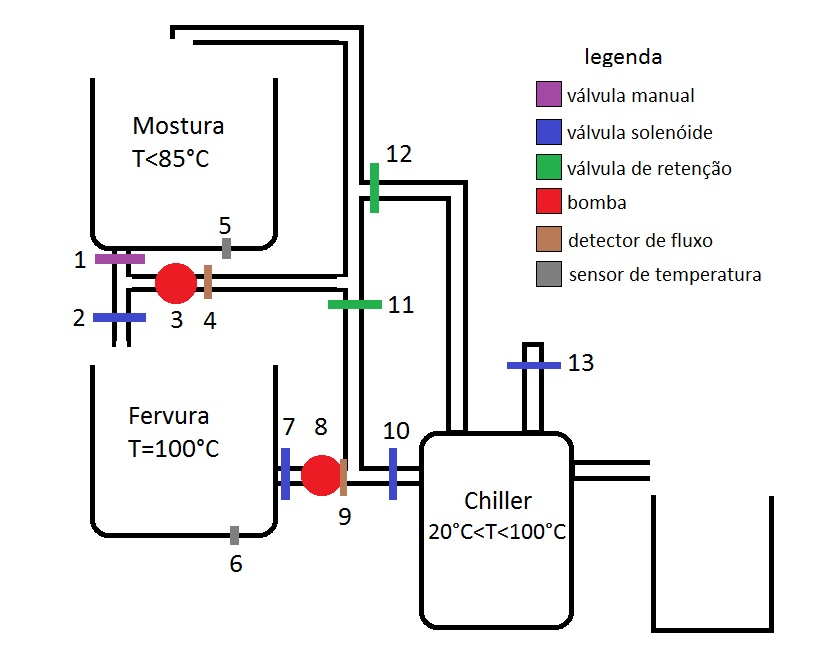
\includegraphics[scale=0.55]{./Resources/esb_mec.jpg}
	\captionsetup{justification=centering}
	\caption[Representação esquemática da estrutura mecânica]{Representação esquemática da estrutura mecânica}
	\label{esboco}
\end{figure}

Na panela superior ou MT, rotulada como \textit{Mostura}, os grãos são adicionados após o aquecimento inicial da água:

\begin{itemize}
	\item A válvula 1 é uma válvula manual do tipo esfera, com passagem plena. Durante a operação do equipamento ela deve ficar sempre aberta, portanto seu uso é realizado somente em caso de emergências.
	\item Após a adição dos grãos, a bomba 3 é ligada para que o líquido da panela seja recirculado. As válvulas de retenção 11 e 12 não permitem que o líquido passe por elas, portanto sobra somente um caminho possível para este, que é ascender na tubulação até entrar novamente na MT. Note-se que não há válvula automatizada na saída da MT, uma vez que o mosto fica em recirculação constante ao longo do processo de cozimento.
	\item Após a mostura a bomba 3 é desligada e a válvula solenóide 2 é aberta, escoando o líquido para a panela de fervura BK. Simultâneamente, a válvula solenóide 7 e a bomba 8 são ativadas, fazendo com que a água de lavagem presente na BK/HLT flua pela tubulação até a MT, iniciando o processo de \textit{sparging}. Durante um tempo predefinido, o mosto e a água de lavagem recirculam pelas duas panelas e se misturam.
	\item Durante a fervura, as válvulas 2 e 7 são fechadas. Neste período a MT deve ser esvaziada, já que ela será usada posteriormente para armazenamento da água de esfriamento do mosto --- água usada para limpeza do sistema e que reduz a produção de efluentes do mesmo.
	\item Após a fervura, as válvulas solenóides 7 e 10 são ativadas, permitindo o escoamento do líquido para o trocador de calor. Simultâneamente a válvula solenóide 13 é aberta e água fria circula em contra-fluxo para resfriar o mosto. Esta água sai quente do trocador de calor e passa pela válvula de retenção 12, preenchendo a parte superior da tubulação e sendo armazenada na MT para posterior limpeza do sistema.
	\item O mosto que sai resfriado do \textit{chiller} cai no balde de fermentação. Neste processo o líquido entra em contato com o ar, o que é não somente desejável como essencial para o sucesso da fermentação, portanto esta é a última parte do processo automatizada. Uma solução futura e que permite automação é o uso de um aerador em conjunto com um tanque de fermentação selado.
\end{itemize}

Para o bom funcionamento do sistema proposto, algumas condições devem ser atendidas:

\begin{itemize}
	\item Se o volume total de líquido nas duas panelas ao final da mostura exceder o volume da BK, ela transbordará. Por este motivo é importante que exista um sistema de detecção de transbordo. Ainda assim, deve-se requisitar que o usuário do sistema calcule corretamente as proporções da receita, pois apesar do sistema automático anti-transbordo, ocorrerá perda de insumos devido ao acúmulo de mosto inutilizável na MT em caso de erro.
	\item São necessários filtros de material particulado para o bom funcionamento das válvulas e bombas \cite{danfoss_solenoid}.
	\item Os dispositivos mecânicos (válvulas, bombas, tubulação, dentre outros) e eletrônicos (sensores e atuadores) em contato com o sistema mecânico devem ser apropriados às altas temperaturas impostas pela natureza do processo \cite{danfoss_solenoid, jefferson_solenoid}.
	\item As panelas, tendo como referência seu fundo, não devem ser alinhadas concêntricas, já que isto torna a adição de lúpulos e o processo de manutenção do equipamento desajeitados.
	\item A automação da técnica de \textit{whirlpool} não é contemplada nesta configuração de sistema. Se o usuário a considera necessária, ele deve se encarregar de executá-la manualmente.
	\item A única válvula com pressão suficiente para ser servo-operada é a 13, assumindo-se que a pressão incidente sobre ela seja maior do que 0,5bar, portanto as outras devem ser de operação direta \cite{danfoss_solenoid, jefferson_solenoid}.
	\item A limpeza automatizada, ou CIP, não é contemplada nesta configuração do sistema, devido à alta complexidade \cite{cip_pres}, conforme indica a figura \ref{cip_system}, e ao custo de implementação proibitivo para este trabalho. Não obstante, é recomendado ao usuário do sistema que faça a limpeza do mesmo tão rápido quanto possível após o final da produção.
\end{itemize}

\begin{figure}[H]
	\centering
	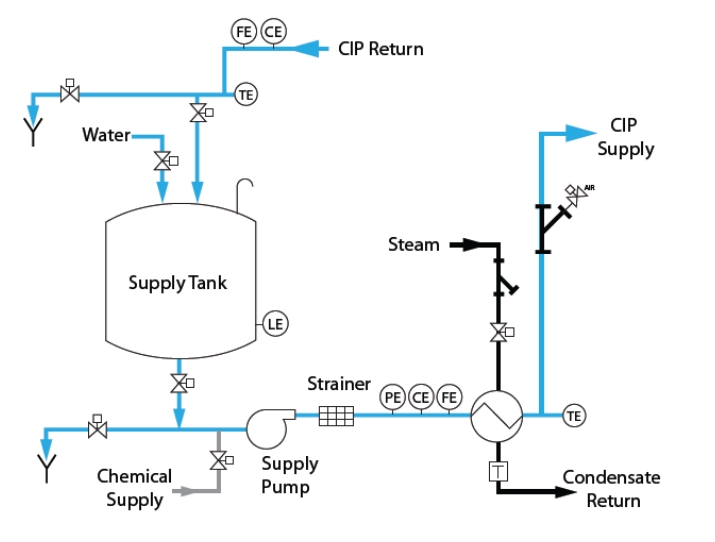
\includegraphics[scale=0.55]{./Resources/cip_example.jpg}
	\captionsetup{justification=centering}
	\caption[Sistema CIP básico]{Sistema CIP básico. \\Fonte: ROSE e MONTGOMERY (2010)}
	\label{cip_system}
\end{figure}

\subsubsection{Dimensionamento da parte funcional} 

Com a filosofia de operação do sistema mecânico definida, é possível realizar o dimensionamento deste sistema. A primeira consideração a ser feita é que os materiais e métodos aqui empregados não seguem nenhuma norma que permita o uso deste equipamento para fabricação de cerveja para venda --- tal escolha é feita em função do alto custo de um sistema completamente dentro das normas e também pelo fato de este ser um trabalho cujo foco é a automação e o acesso remoto.

Não obstante, o material da tubulação escolhido foi o aço inoxidável AISI304. Já que o volume de líquido a ser trabalhado é pequeno, menor do que 40 litros, e a pressão de trabalho não é maior do que a pressão das bombas escolhidas posteriormente, foi decidido o uso de tubulação de diâmetro de 1/2" (21,34mm de diâmetro externo) e espessura da parede no padrão Schedule 40 (2,77mm de espessura). Embora esta espessura seja superdimensionada para a presente aplicação, o mecânico responsável pela montagem do sistema a requisitou para que fosse possível fazer rosca sem danificar a integridade dos tubos. As conexões, seguindo a escolha dos tubos, também são de aço inoxidável de 1/2".

As ligações entre tubos, conexões e outros componentes do sistema são ligações rosqueadas. Este é um meio de ligação antigo, porém de baixo custo, fácil execução e usualmente empregadas em tubulações de diâmetro nominal pequeno, menor do que 4" \cite{ifba}. Para vedação foi escolhido o Teflon, uma vez que é um material de baixo custo e alta disponibilidade e o padrão de rosca adotado neste projeto é o BSP, baseado na norma ISO. Cabe salientar que, embora as ligações rosqueadas sejam permitidas sob certas circunstâncias na prática, elas são relegadas a instalações de baixa responsabilidade \cite{ifba}.

As panelas foram escolhidas no material de alumínio, em função do custo proibitivo do aço inoxidável. São caldeirões padrão utilizados no ramo de hotelaria e restaurantes e disponíveis em vários volumes. As duas panelas utilizadas neste trabalho tem capacidade para 32 litros e diâmetro do fundo de 36cm, portanto sua especificação no mercado é \textit{caldeirão de alumínio n. 36}. Tal volume, 60\% superior ao da produção máxima aconselhada, é necessário devido ao volume dos grãos, à quantidade da água de lavagem e às perdas por evaporação que exigem uso de um volume de água inicial superior ao nominal.

O parâmetro inicial escolhido para seleção das válvulas solenóide foi a temperatura máxima de operação, cuja fonte de dados de operação é fornecida pelos fabricantes. Em seguida, foi escolhida uma vedação adequada: os dois tipos mais comums de vedação com suporte a temperatura de pelo menos 100\si{\degree}C são o EPDM e FKM (etileno-propileno-dieno e fluoreto de vinilideno, respectivamente) \cite{danfoss_solenoid}. Estes materiais possuem uma tabela de compatibilidade de fluidos cuja classificação pode ser satisfatória, boa, duvidosa, insatisfatória e desconhecida --- tanto para cerveja quanto para o mosto, ambas as vedações são classificadas como satisfatórias, embora para água a classificação do FKM seja somente boa \cite{epdm_fkm}. Por fim, um parâmetro que foi verificado antes da escolha final das válvulas é a posição de operação, que varia conforme os modelos do fabricante \cite{danfoss_solenoid}. Com base nos parâmetros supracitados, foi decidido usar:

\begin{itemize}
	\item Válvula solenóide 1/2" 12V plástico uso geral para água de resfriamento do trocador de calor.
	\item Válvula solenóide Danfoss 1/2" EV210BD 032U3620 para demais válvulas.
	\item Bobina Danfoss 15W 12VDC 042N7550 para acionamento das solenóides Danfoss.
\end{itemize}


Informações técnicas sobre a válvula EV210BD 032U3620 estão no anexo \ref{Anexo3} e sobre a bobina 042N7550 no anexo \ref{Anexo4}.

As bombas de recirculação foram escolhidas com base na temperatura de operação e grau alimentício. Posteriormente, tanto a vazão quanto a perda de carga do sistema foram estimadas para verificar se a bomba escolhida seria adequada: o modelo Topsflo B08H-12-1006 tem capacidade máxima de vazão de 10l/min e carga expressa em coluna de água de 6m. Como a capacidade máxima do sistema é de 20l e idealmente a temperatura deve subir à taxa de 1\si{\degree}C/min, além de que a altura do sistema é menor do que 2m e as perdas de carga foram consideradas desprezíveis para este caso, foi decidido que a bomba escolhida é adequada ao projeto. No \ref{Anexo5} encontra-se a folha de dados tećnicos do dispositivo.

Quanto às conexões, a figura \ref{conexoes_rascunho} apresenta um diagrama conceitual do sistema, contendo todas as peças necessárias para a montagem do mesmo:

\begin{figure}[H]
	\centering
	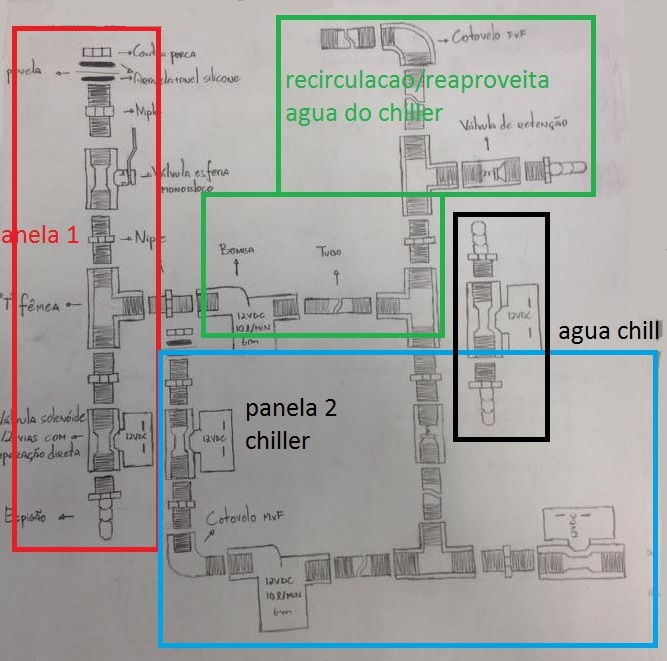
\includegraphics[scale=0.55]{./Resources/conexoes.jpg}
	\captionsetup{justification=centering}
	\caption[Diagrama conceitual das conexões mecânicas]{Diagrama conceitual das conexões mecânicas}
	\label{conexoes_rascunho}
\end{figure}

Na figura \ref{mt_cad} é apresentado um diagrama da MT construído no software FreeCAD, à qual estão conectados o resistor de potência e um niple com vedação. Também estão presentes na figura a válvula esfera manual, um \textit{tee} fêmea, uma válvula Danfoss EV210B e três niples de conexão entre estes componentes. O modelo da válvula foi obtido a partir do website da Danfoss e importado, enquanto a modelagem dos outros componentes foi desenvolvida na plataforma FreeCAD. Na figura \ref{mt_cad_close} são apresentadas em detalhe as conexões do resistor e do niple à panela e, por isto, a estrutura da mesma foi omitida. Os itens em amarelo são contra-porcas, em azul arruelas e, em vermelho anéis de vedação (\textit{o-rings}).

\begin{figure}[H]
	\centering
	\begin{subfigure}{.46\textwidth}
		\centering
		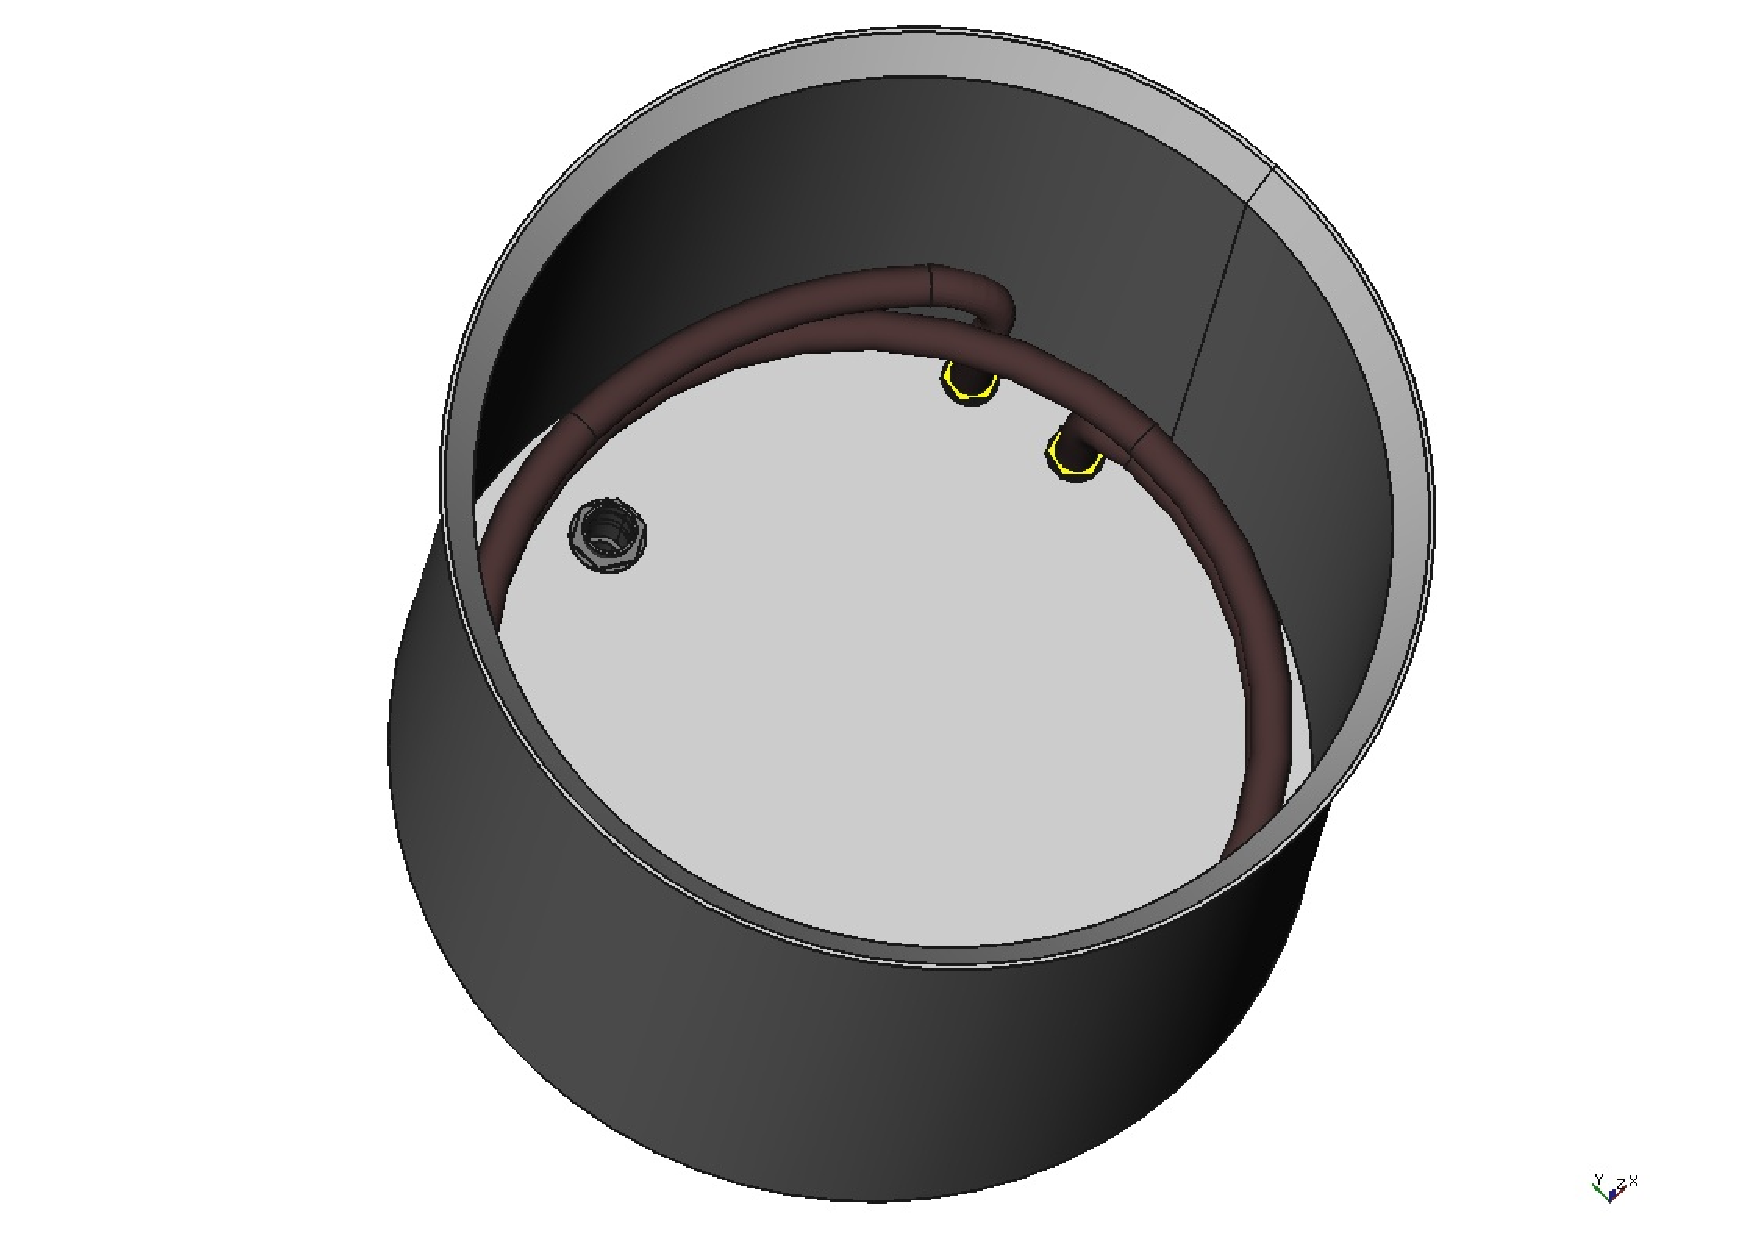
\includegraphics[height=8cm]{./Resources/mecsys/mash-tun-top-color.pdf}
		\caption{Vista superior}
		\label{mt_cad:1}
	\end{subfigure}
	\begin{subfigure}{.46\textwidth}
		\centering
		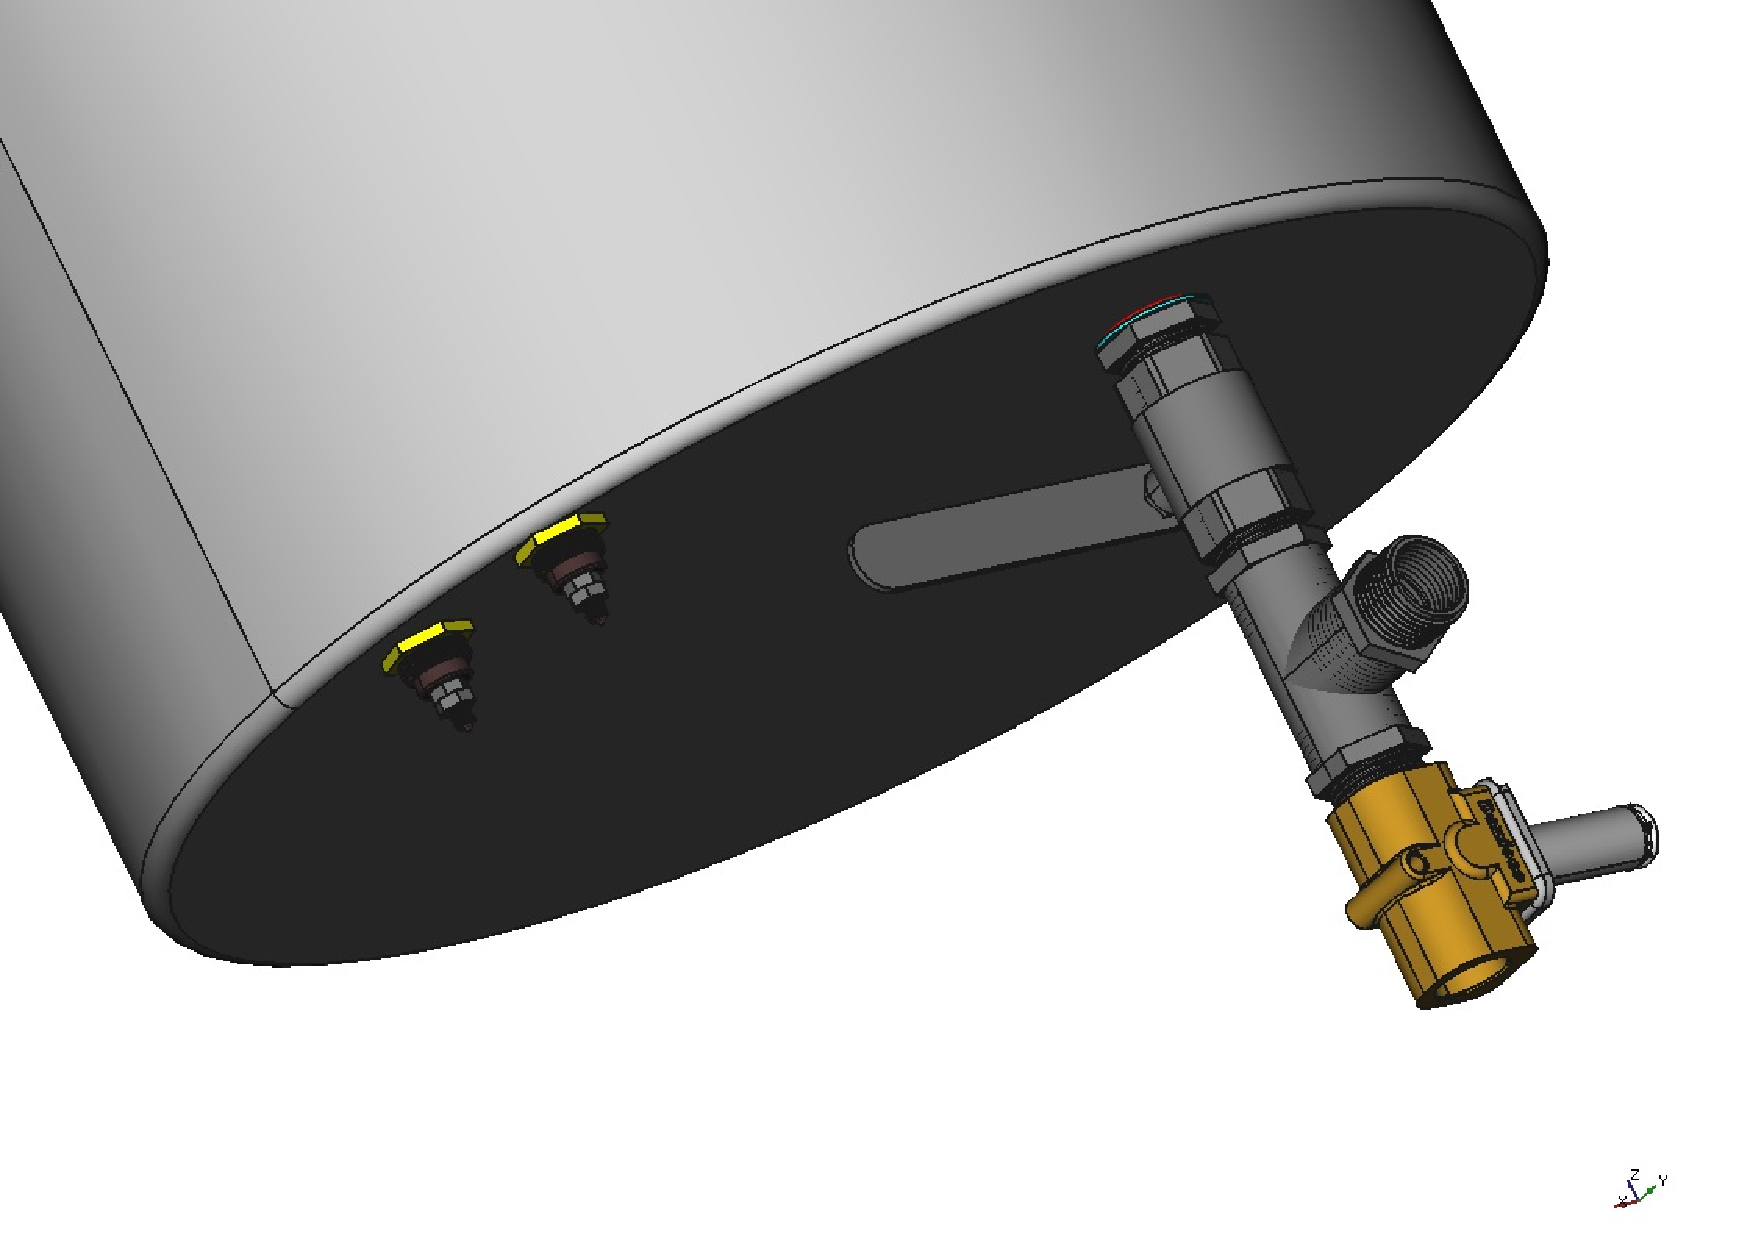
\includegraphics[height=8cm]{./Resources/mecsys/mash-tun-bottom-color.pdf}
		\caption{Vista inferior}
		\label{mt_cad:2}
	\end{subfigure}
	\captionsetup{justification=centering}
	\caption[Diagrama da panela de mostura e conexões]{Diagrama da panela de mostura e conexões}
	\label{mt_cad}
\end{figure}

\begin{figure}[H]
	\centering
	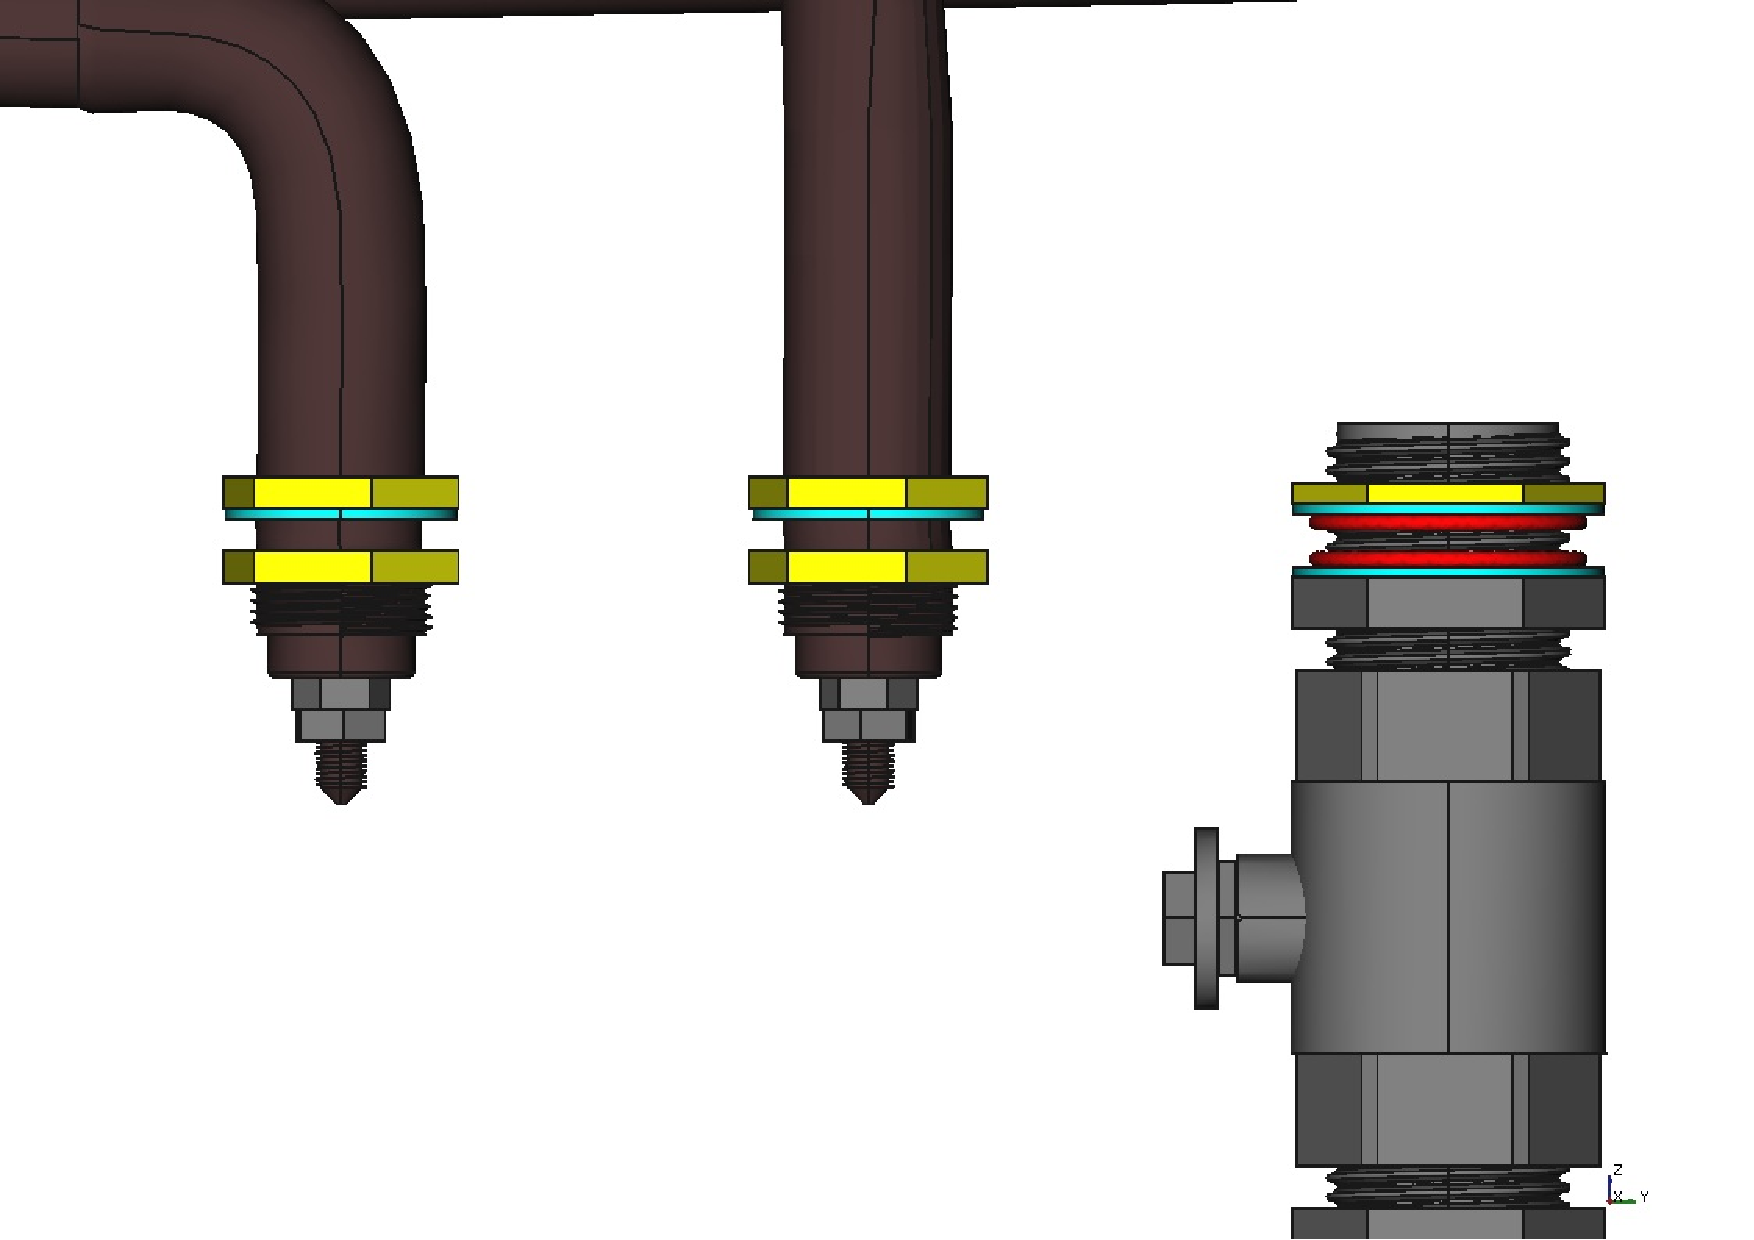
\includegraphics[scale=0.55]{./Resources/mecsys/mash-tun-seal-color.pdf}
	\captionsetup{justification=centering}
	\caption[Detalhes da vedação da panela de mostura]{Detalhes da vedação da panela de mostura}
	\label{mt_cad_close}
\end{figure}

\subsubsection{Estrutura metálica de suporte}

Parte importante do projeto foi o dimensionamento da estrutura metálica de suporte às panelas, já que esta é responsável não somente pelo bom funcionamento do sistema mecânico como também pela facilidade de manutenção do mesmo.



\subsection{Configuração da BeagleBone Black}

O primeiro passo para o desenvolvimento do projeto foi a configuração da BeagleBone Black, que é o coração deste sistema. Para tal, foi escolhido o procedimento de gravar a distribuição Debian pré-compilada do sistema operacional Linux na memória de armazenamento eMMC de 4GB da placa. Esta distribuição foi escolhida em função da facilidade de obtenção de suporte em fóruns da internet, artigos e livros, dentre outros, além de ser o SO oficial da BBB \cite{bbb_debian}.

NOTA: Na ocasião da realização deste procedimento, havia uma diferenciação entre a imagem fornecida para uso diretamente a partir do cartão \si{\micro}SD e a imagem para gravação no eMMC, porém agora o procedimento adotado pela fundação BeagleBoard.org é fornecer somente uma imagem pronta para uso diretamente do cartão \si{\micro}SD e, no caso de o usuário decidir gravar a distribuição no eMMC, o arquivo uEnv.txt na partição de \textit{boot} do cartão \si{\micro}SD deve ser editado conforme instruções antes de ser inserido na BBB.

Tanto a última versão estável do Debian para BBB (v. 7.9), conhecida como \textit{Wheezy} e a última versão em desenvolvimento (v. 8.2), conhecida como \textit{Jessie}, quanto a versão utilizada neste projeto (v. 7.5) podem ser obtidas a partir do site oficial da BBB \cite{bbb_images}, conforme ilustrado na figura \ref{debian_images}. A instalação da versão 7.5 se resume a:

\begin{enumerate}
	\item Baixar a imagem Debian 7.5 para eMMC do site \url{beagleboard.org/latest-images}
	\item Descomprimir a imagem
	\item Gravar a imagem em um cartão \si{\micro}SD formatado (não basta copiar, é preciso utilizar um software que grave a imagem corretamente. Neste caso foi utilizado o \textit{Win32 Disk Imager})
	\item Inserir o cartão \si{\micro}SD na BBB desligada
	\item Pressionar o botão de boot e energizar a placa com ele ainda pressionado
	\item Esperar um dos leds de status acender antes de largar o botão
	\item Esperar os 4 leds de status ficarem continuamente acesos (durante o processo de gravação eles trabalharão de maneira intermitente)
	\item Desenergizar a BBB e retirar o cartão \si{\micro}SD
\end{enumerate}
 
 \newpage
 
\begin{figure}[H]
	\centering
	\fbox{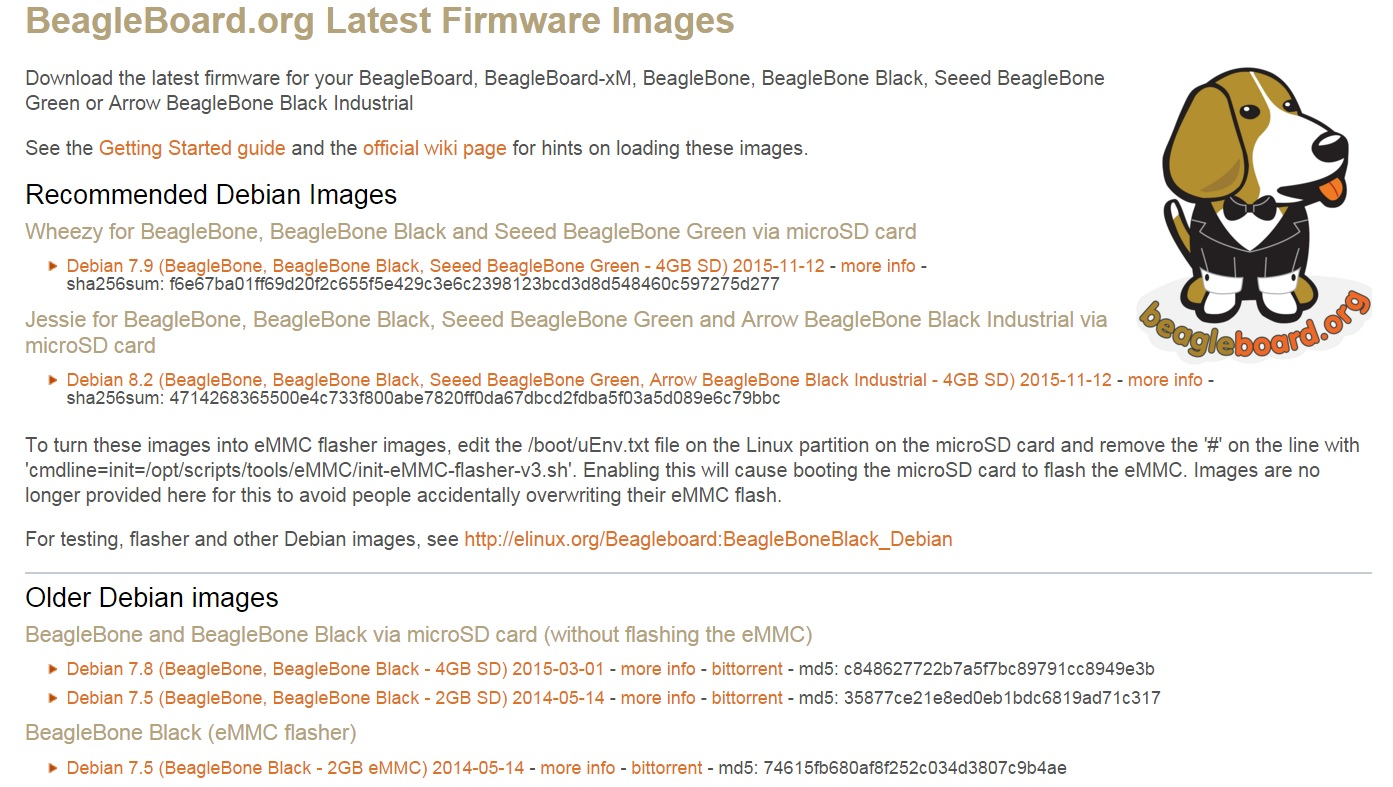
\includegraphics[scale=0.30]{./Resources/debian-latest.jpg}}
	\captionsetup{justification=centering}
	\caption[Últimas imagens pré-compiladas disponíveis para a BBB]{Últimas imagens pré-compiladas disponíveis para a BBB. \\Fonte: Adaptado do site oficial da Fundação BeagleBoard.org\protect\footnotemark}
	\label{debian_images}
\end{figure}

\footnotetext{Disponível em \url{http://beagleboard.org/latest-images}}

Após este procedimento, a BBB estará pronta para uso a partir da memória interna eMMC. A verificação do funcionamento do sistema foi feita conectando a placa a um computador instalado com Windows 7 e conectado à internet, via interface USB e posterior acesso através do software de código aberto para acesso via SSH \textit{Putty}, disponível para \textit{download} no site oficial \url{putty.org} \cite{putty} (qualquer software similar que possibilite o acesso via SSH pode ser utilizado para este fim). Para isso, é preciso também instalar no computador o driver que dá acesso à BBB via USB, disponível em \url{beagleboard.org/getting-started}. O acesso via SSH se dá utilizando o endereço de IP \textbf{192.168.7.2}, usuário: \textbf{debian} e senha: \textbf{debian} \cite{lumme}. A figura \ref{putty-cfg} mostra o ambiente de configuração do \textit{Putty} e a figura \ref{putty-flogin} apresenta a tela após uma tentativa de login bem sucedida.

\begin{figure}[H]
	\centering
	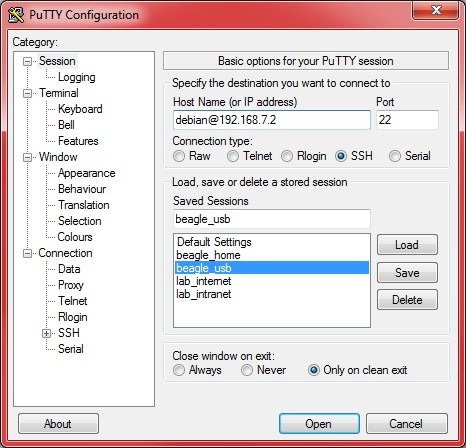
\includegraphics[scale=0.90]{./Resources/putty-cfg.jpg}
	\captionsetup{justification=centering}
	\caption[Configuração do \textit{Putty} para acesso SSH via USB]{Configuração do \textit{Putty} para acesso SSH via USB}
	\label{putty-cfg}
\end{figure}

\begin{figure}[H]
	\centering
	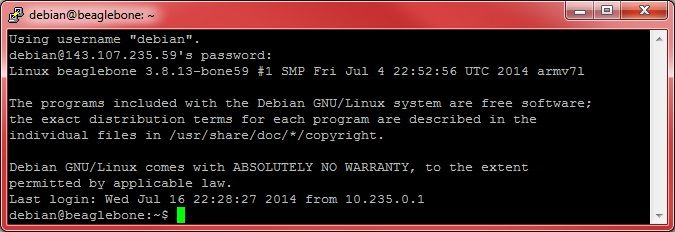
\includegraphics[scale=0.80]{./Resources/putty-first-login.jpg}
	\captionsetup{justification=centering}
	\caption[Tentativa de login bem sucedida pelo \textit{Putty}]{Tentativa de login bem sucedida pelo \textit{Putty}}
	\label{putty-flogin}
\end{figure}

\subsubsection{Configuração da rede para uso do adaptador Wi-Fi/USB}

Para utilizar o adaptador Wi-Fi USB, em primeiro lugar este foi conectado à BBB. Em seguida, no terminal, o dispositivo foi listado para confirmar que o sistema estava identificando-o corretamente e ativado, permitindo assim obter a lista de redes Wi-Fi próximas. Com isso, foi possível obter os dados da rede Wi-Fi de interesse, para posterior edição do arquivo \textit{/etc/network/interfaces}, responsável pelas configurações de rede do sistema -- este pode ser obtido no apêndice \ref{Apêndice B}. O código abaixo ilustra a sequência de comandos executados:

\lstset{language=bash}
\begin{lstlisting}[frame=single, basicstyle=\linespread{0.85}\ttfamily]
	lsusb # verifica se o dispositivo USB foi detectado
	sudo ifconfig wlan up # ativa a interface de rede USB
	sudo iwlist scan # lista as redes Wi-Fi disponíveis
	
	# Identificar os valores da rede de interesse, e.g.
	#	ESSID:"Nome_da_rede" -> nome da rede
	#	IE: IEEE 802.11i/WPA2 Version 1 -> encriptação
	# E então é modificado o arquivo de configuração
	
	# abre o arquivo para edição
	sudo nano /etc/network/interfaces 
	# Após modificar o arquivo e salvá-lo:
	
	sudo ifup wlan0 # ativa a interface de rede Wi-Fi
	sudo ifdown eth0 # desativa a interaface Ethernet

\end{lstlisting}

No arquivo \textit{/etc/network/interfaces}, as configurações utilizadas entre as linhas 19 e 35 do código são referentes à configuração do Wi-Fi para configuração da BBB com endereço de IP estático, permitindo o acesso à plataforma remotamente pela internet e não somente dentro da intranet. Depois de todo este procedimento, o dispositivo ainda não estava funcionando após a operação de \textit{reboot}, portanto foi utilizado um \textit{script} de reset do Wi-Fi executado durante o \textit{boot}, cujas instruções de uso, obtidas em  \url{https://learn.adafruit.com/setting-up-wifi-with-beaglebone-black/configuration}, foram as seguintes:

\lstset{language=bash}
\begin{lstlisting}[frame=single, basicstyle=\linespread{0.85}\ttfamily]
git clone https://github.com/adafruit/wifi-reset.git #download do script
cd wifi-reset/ #entra no diretório do script
chmod +x install.sh #permissão de execução para o script
sudo ./install.sh #executa o script
\end{lstlisting}

\subsubsection{Configuração de data/hora}

Para a configuração automática de data e hora da BBB, foi escolhido o uso do protocolo NTP -- \textit{Network Time Protocol} ou Protocolo de Tempo para Redes -- cujo objetivo é sincronizar os relógios de dispositivos conectados a uma rede a partir de fontes precisas \cite{ntp}. No Brasil, a confiabilidade deste protocolo é responsabilidade do Observatório Nacional (ON), responsável legal por garantir a Hora Legal Brasileira, em conjunto com o Núcleo de Informação e Coordenação do Ponto BR, administrador e operador do domínio ".br"  \cite{nic,dsho}.

Primeiramente foi realizada a instalação do protocolo, seguida da configuração do arquivo \textit{/etc/ntp.conf} e da modificação do arquivo que indica a \textit{timezone}, sendo este um link simbólico para o verdadeiro arquivo. Os comandos executados estão descritos abaixo:

\lstset{language=bash}
\begin{lstlisting}[frame=single, basicstyle=\linespread{0.85}\ttfamily]
sudo apt-get install ntp #instala o NTP
sudo nano /etc/ntp.conf #abre o arquivo de configuração para edição
sudo mv /etc/localtime /etc/localtime-old #backup do arquivo antigo da timezone
sudo ln -s /usr/share/zoneinfo/America/Sao_Paulo /etc/localtime #cria link simbólico para arquivo da nova timezone
\end{lstlisting}

Na edição do arquivo \textit{/etc/ntp.conf}, a única modificação feita é a substituição dos servidores de hora padrão para os servidores brasileiros, listados no endereço \url{http://www.pool.ntp.org/zone/br} -- no final de cada endereço foi adicionada a instrução \textit{iburst}, conforme descrito no website oficial do protocolo (\url{http://support.ntp.org/bin/view/Support/ConfiguringNTP}) e que, embora não esteja claro seu funcionamento, é essencial para que o horário seja corretamente configurado a cada \textit{reboot}. O trecho de código modificado no arquivo \textit{/etc/ntp.conf} com os servidores brasileiros é ilustrado abaixo:

\lstset{language=bash}
\begin{lstlisting}[frame=single, basicstyle=\linespread{0.85}\ttfamily]
# You do need to talk to an NTP server or two (or three).
#server ntp.your-provider.example

# pool.ntp.org maps to about 1000 low-stratum NTP servers. Your server will
# pick a different set every time it starts up. Please consider joining the
# pool: <http://www.pool.ntp.org/join.html>
server 0.br.pool.ntp.org iburst
server 1.br.pool.ntp.org iburst
server 2.br.pool.ntp.org iburst
server 3.br.pool.ntp.org iburst
\end{lstlisting}

%%%%%%%%%%%%%%%%%%%%%%%%%%%%%%%%%%%%%%%%%%%%%%%%%%%%%%%%%%%%%%%%%%%%%%%%%%

\subsection{Aplicação \textit{server-side} em Node.js}

\subsection{Interface de usuário}

A interface de usuário foi desenvolvida para acesso via navegador da internet. Dois servidores foram utilizados em conjunto: o servidor Apache, que é um servidor \textit{web} robusto e de fácil implementação e o \textit{framework Express.js}, para \textit{Node.js}. As linguagens utilizadas para a implementação da aplicação foram: a linguagem de marcação HTML, a linguagem de folhas de estilo CSS, a linguagem de programação \textit{client-side} interpretada Javascript em conjunto com a biblioteca \textit{crossbrowser} jQuery e o método AJAX, a linguagem de programação \textit{server-side} interpretada PHP e, a linguagem de programação \textit{server-side} Javascript interpretada pela aplicação \textit{Node.js}.

Parte da implementação foi feita por meio de acesso ao terminal via SSH e parte via \textit{Cloud9}, que é uma IDE online. A estrutura da aplicação desenvolvida é apresentada:

\begin{itemize}
	\item Página inicial
	\item Página de apresentação
	\item Gráficos de temperatura dinâmico e estático (página somente para versão de demonstração)
	\item Menu de seleção de tarefas
	\begin{itemize}
		\item Gerenciador de receitas de cerveja
		\begin{itemize}
			\item Editor de receitas
		\end{itemize}
		\item Gerenciador de início da produção (em desenvolvimento)
		\item Acompanhamento e possibilidade de ajustes da brassagem (em desenvolvimento)
		\item Estatísticas (a ser desenvolvida)
		\item Opções e ajuste de configurações do sistema (a ser desenvolvida)
	\end{itemize}
\end{itemize}

Os códigos desenvolvidos e comentados podem ser consultados no apêndice \ref{Apêndice B} e os resultados são descritos na seção \ref{resIntUser}.

\subsection{Circuitos de interface}

\subsection{Sistema de controle de temperatura}

